% https://www.overleaf.com/learn/latex/page_size_and_margins
%
% arr: move draw to two tikz environments not document
%	change paper size with geometry
% add manual way of creating a cuboid

\documentclass{article}
\usepackage{geometry}
\geometry{
	a5paper,
	left=10mm,
	top=20mm,
} 

\usepackage{tikz}

\newcommand{\tikzcuboid}[4]{% width, height, depth, scale
	% define tikz object
	\begin{tikzpicture}[scale=#4]
		\foreach \x in {0,...,#1}
		{   \draw (\x ,0  ,#3 ) -- (\x ,#2 ,#3 );
			\draw (\x ,#2 ,#3 ) -- (\x ,#2 ,0  );
		}
		\foreach \x in {0,...,#2}
		{   \draw (#1 ,\x ,#3 ) -- (#1 ,\x ,0  );
			\draw (0  ,\x ,#3 ) -- (#1 ,\x ,#3 );
		}
		\foreach \x in {0,...,#3}
		{   \draw (#1 ,0  ,\x ) -- (#1 ,#2 ,\x );
			\draw (0  ,#2 ,\x ) -- (#1 ,#2 ,\x );
		}
	\end{tikzpicture}
}

\newcommand{\tikzcube}[2]{% length, scale
	\tikzcuboid{#1}{#1}{#1}{#2}
}


\begin{document}
	
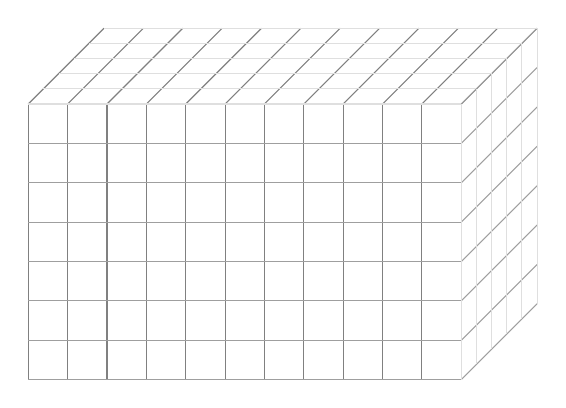
\begin{tikzpicture}[scale=0.5]
	% manual way of creating a cuboid drawing lines
	\foreach \x in {0,...,11}
	{   \draw[gray] (\x, 0, 5 ) -- (\x, 7, 5 );
		\draw[gray] (\x, 7, 5 ) -- (\x, 7, 0 );
	}
	\foreach \x in {0,...,7}
	{   \draw[gray!75] (11, \x, 5) -- (11, \x, 0);
		\draw[gray!75] (0, \x, 5) -- (11, \x, 5);
	}
	\foreach \x in {0,...,5}
		{   \draw[gray!25]  (11, 0, \x ) -- (11, 7, \x);
			\draw[gray!25]  (0, 7, \x) -- (11, 7, \x);
	}
\end{tikzpicture}

\vspace{35pt}

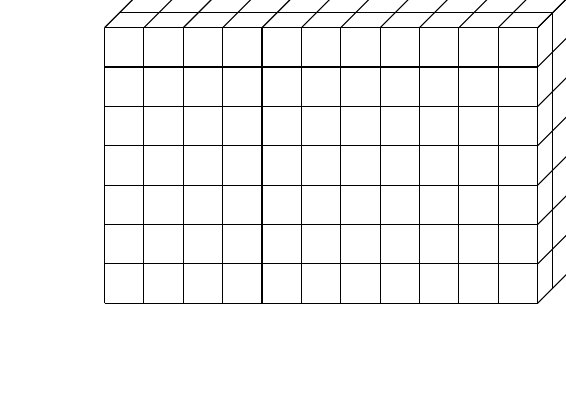
\begin{tikzpicture}
	\tikzcuboid{11}{7}{5}{0.5}
\end{tikzpicture}

\vspace{20pt}

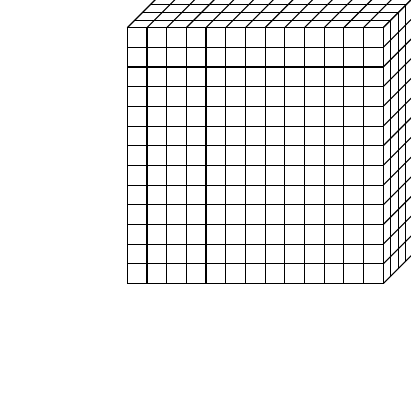
\begin{tikzpicture}
	\tikzcube{13}{0.25}
\end{tikzpicture}

\end{document}
